% A test document for daarticle.cls: an excerpt of
%   D. Avitabile, Projection methods for neural field equations,
%   SIAM J. Numer. Anal. (2023).
% It exercises the features a paper needs: title block, abstract, keywords,
% MSC codes, sections, hypotheses, theorems, lemmas and proofs, displayed and
% aligned equations, cross-references, citations, a figure, a table and an
% appendix. Switch the \documentclass line to compare with the SIAM classes.
% \documentclass[a4paper]{siamart251216}
% \documentclass[a4paper]{siamonline250211}
\documentclass[a4paper,baskervaldx]{daarticle}
% \documentclass[a4paper]{daarticle}

\usepackage{damacros}
\usepackage{booktabs}
\renewcommand{\phi}{\varphi}
\newcommand{\rev}[1]{#1}
\newcommand{\linelabel}[1]{}
\newcommand{\otoprule}{\midrule[\heavyrulewidth]}
\graphicspath{{./Figures/}}

% Sets running headers as well as PDF title and authors
\headers{Projection methods for Neural Field equations}{D. Avitabile}

% Title
\title{Projection methods for Neural Field equations} 

% Authors: full names plus addresses.
\author{%
  Daniele Avitabile%
  \thanks{%
    Vrije Universiteit Amsterdam,
    Department of Mathematics,
    Faculteit der Exacte Wetenschappen,
    De Boelelaan 1081a,
    1081 HV Amsterdam, The Netherlands.
  \protect\\
    Inria Sophia Antipolis M\'editerran\'ee Research Centre,
    MathNeuro Team,
    2004 route des Lucioles-Boîte Postale 93 06902,
    Sophia Antipolis, Cedex, France.
  \protect\\
    (\email{d.avitabile@vu.nl}, \url{www.danieleavitabile.com}).
  }%
}

\begin{document}

\maketitle

\begin{abstract}
  Neural field models are nonlinear integro-differential equations for the evolution
  of neuronal activity, and they are a prototypical large-scale, coarse-grained
  neuronal model in continuum cortices. Neural fields are often simulated
  heuristically and, in spite of their popularity in mathematical neuroscience,
  their numerical analysis is not yet fully established. We introduce generic
  projection methods for neural fields, and derive a-priori error bounds for these
  schemes. We extend an existing framework for
  stationary integral equations to the time-dependent case, which is relevant for
  neuroscience applications. We find that the convergence rate of a projection scheme for a
  neural field is determined to a great extent by the convergence rate of the
  projection operator. This abstract analysis, which unifies the treatment of
  collocation and Galerkin schemes, is carried out in operator form, without
  resorting to quadrature rules for the integral term, which are
  introduced only at a later stage, and whose choice is enslaved by the choice of the
  projector. Using an elementary timestepper as an example, we demonstrate that the
  error in a time stepper has two separate contributions: one from the projector, and
  one from the time discretisation. We give examples of concrete projection methods: two
  collocation schemes (piecewise-linear and spectral collocation) and two Galerkin
  schemes (finite elements and spectral Galerkin); for each of them we derive error
  bounds from the general theory, introduce several discrete variants, provide
  implementation details, and present reproducible convergence tests.
\end{abstract}

\begin{keywords}
  neural fields, projection methods, collocation, Galerkin, error bounds
\end{keywords}

\begin{MSCcodes}
  65R20, 45K05, 92C20
\end{MSCcodes}

\section{Introduction}\label{sec:model}
Neural field models are integro-differential equations describing the
spatially-extended, coarse-grained activity of neurons in continuum cortices. The
simplest and most studied neural field model is written as
\begin{equation} \label{eq:NF}
  \begin{aligned}
  & \partial_t u(x,t) = -u(x,t) + \int_\Omega w(x,y) f(u(y,t))\, dy + \xi(x,t), \qquad
    && (x,t) \in \Omega \times J \\
  & u(x,t_0) = u_0,                         
    && x \in \Omega.
  \end{aligned}
\end{equation}
where $u(x,t)$ is the voltage of a neuronal population at time
$t$ and point $x$ in the cortex $\Omega$, which is a compact domain in
$\mathbb{R}^d$.
%
The function $w(x,y)$ is
the \emph{synaptic kernel}, modelling synaptic strengths from point $y$ to point
$x$ in the tissue, whereas $f$ is the \emph{firing rate} of the population; the
function $\xi$ models an external input. Finally, $J$ is a time interval
\linelabel{line:negTime1} \rev{containing $t_0$, typically $J = [t_0,t_0+T]$ or $J=[t_0-T,t_0+T]$}. Intuitively, the first term in the
right-hand side of the evolution equation in \cref{eq:NF} models local decay, while
the integral term collects inputs from the whole cortex. Typically the function $f$
is taken to be a steep, bounded sigmoidal function (approximating a Heaviside step
function), hence a neuronal patch in $y$ contributes to the activity in $x$
nonlinearly, and only if its voltage is sufficiently high.

Since their introduction by Wilson and Cowan~\cite{wilson1973mathematical}, and
Amari~\cite{amari1977dynamics}, neural fields have
been used to analyse and reproduce macroscopic cortical patters of activity,
including localised stationary bumps, travelling waves and spiral waves. As discussed
in several mathematical neuroscience reviews and textbooks 
\cite{Ermentrout.1998qno,Ermentrout.2010,Bresloff.2012,
Bressloff.2014k0p,coombes2014neural}, the model
\cref{eq:NF} can be extended in many ways, including multiple neuronal
populations, stochastic forcing, and distributed delays. 


This document is an excerpt of the paper above, kept to test the document
class: in \cref{sec:prelim} we cast \cref{eq:NF} as a Cauchy problem on Banach
spaces, projection methods are introduced in \cref{sec:projection_methods}, and
\cref{sec:numerics} shows convergence tests for a few schemes, with the problems
listed in \cref{tab:parameters}. Proofs of the auxiliary results are in the
appendix.

\subsection{Notation}
We denote by $C(\Omega,\RSet)$ or $C(\Omega)$ the space of
real-valued continuous function defined on $\Omega$, with the supremum norm $\|
\blank \|_\infty$. We use $L^2(\Omega,\RSet)$ or $L^2(\Omega)$ for the
Hilbert space of real-valued square-integrable functions defined on $\Omega$, with
norm $\| \blank \|_{L^2(\Omega)}$. Since we use both functional settings, we will
often consider $\XSet \in \{C(\Omega),L^2(\Omega)\}$, and write $\| \blank \|$, to
indicate the associated norm. 
%We write $\langle \blank, \blank \rangle$ for the
%standard inner product in $L^2(\Omega)$, and  
We write $\| \blank \|_2$ for the $2$-norm on
$\RSet^n$. In addition, we denote by $B(\RSet)$ the space of bounded functions
defined on $\RSet$, with norm $\| \blank \|_\infty$.
%
We will also indicate by $BL(\XSet,\YSet)$ the space of bounded linear operators from
$\XSet$ to $\YSet$, where $\XSet$ and $\YSet$ are Banach spaces. The space
$BL(\XSet,\YSet)$ is endowed with the operator norm
\[
  \| A \|_{BL(\XSet,\YSet)} = \sup_{x \in \XSet_{\neq 0}} \frac{\| A
  x\|_\YSet}{\| x\|_\XSet}.
\]
We will also abbreviate $\| \blank \|_{BL(\XSet,\YSet)}$ by $\| \blank \|$, when the
context is unambiguous.
%
Since we work often with indices, it is useful to introduce the index sets 
$\NSet_n = \{1, \ldots,n\}$, $\ZSet_{n}= \{0,\ldots,n-1\}$, and $\ZSet_{\pm n}
=\{0,\pm 1,\ldots,\pm n\}$, for a fixed $n \in \NSet$.


\section{Neural field equations as Cauchy problems on Banach spaces} 
\label{sec:prelim} Before introducing the projection schemes, we wish to cast the neural
field equation
\cref{eq:NF} as a Cauchy problem on a Banach space $\XSet \in \{C(\Omega),
L^2(\Omega)\}$. These concrete choices for $\XSet$ are motivated by the functional
setup that are appropriate for collocation and Galerkin schemes, respectively.
%
We collect below our working hypotheses, which hold in standard neural field
models in literature~\cite{Ermentrout.2010,Bressloff.2014k0p,coombes2014neural}.
\begin{hypothesis}[Cortex]\label{hyp:domain}
  The domain $\Omega \subset \RSet^d$ is compact,
  with measure $| \Omega |$.
\end{hypothesis}
 
\begin{hypothesis}[Synaptic kernel]\label{hyp:kernel}
  If $\XSet = L^2(\Omega)$, the synaptic kernel $w$ is a function in $L^2(\Omega
  \times \Omega)$. If $\XSet = C(\Omega)$, we assume that the following holds: 
  \begin{align}
    & \lim_{h \to 0} \omega(h) = 0,  \qquad \omega(h) = \sup_{\substack{x,z \in \Omega\\ \| x- z \|_2 \leq h}} \int_\Omega
    |w(x,y) - w(z,y)|\, dy, \\
    & \sup_{x \in \Omega} \int_\Omega |w(x,y)| \, dy < \infty.
  \end{align}
\end{hypothesis}
%

\begin{hypothesis}[Firing rate]\label{hyp:firingRate}
  The firing rate function $f \colon \RSet \to \RSet$ is a bounded and everywhere
  differentiable Lipschitz function, hence $f,f' \in B(\RSet)$.
\end{hypothesis}

\begin{hypothesis}[External input]\label{hyp:externalInput} The mapping $t \to
  \xi(\blank,t)$ is continuous from $J$ to $\XSet \in \{C(\Omega),L^2(\Omega)\} $.This is written,
  with a slight abuse of notation\footnote{We are using the same symbol, $\xi$, to
  denote a function $\xi \colon \Omega \times J \to \XSet$, and the mapping $t \mapsto
\xi(\blank,t)$ on $J$ to $\XSet$. A similar notation will be also used for $u$.}, $\xi \in C(J,\XSet)$.
\end{hypothesis}

As we shall see in a moment, the hypotheses on the kernel guarantee the compactness
of a suitably defined integral operator $W$ with kernel $w$, which will be defined below \cite[Section
2.8.1]{atkinson2005theoretical}. In passing, we note that any $w \in C(\Omega \times
\Omega)$ satisfies \cref{hyp:kernel}. The firing rate $f$ is required to be
differentiable, thereby excluding the case of Heaviside firing rate, an hypothesis
that is employed in the analytic construction of neural field patterns
\cite[Chapters 1, 3]{amari1977dynamics,coombes2014neural}, but it is
dictated mostly by mathematical convenience, and is less relevant to numerical
simulations.

%
We define the following operators
\begin{align}
  F(u)(x) & := f(u(x)),               & & x \in \Omega, \label{eq:NemOp} \\ 
  (Wu)(x) & := \int_\Omega w(x,y) u(y)\, dy, & & x \in \Omega, \label{eq:WOp} \\
  K(u)(x) & := (WF(u))(x),         & & x \in \Omega, \label{eq:KOp}
\end{align}
and we rewrite \cref{eq:NF} formally, as
\[
  \begin{aligned}
    & u'(t) = N(t,u(t)):=-u(t) + K(u(t)) + \xi(t) \qquad & t \in J, \\
    & u(t_0) = u_0.
  \end{aligned}
\]
The system above is the sought Cauchy problem on the Banach space $\XSet$; this
section is devoted to make this step more precise, and to present bounds useful in
upcoming calculations.
%
%\subsection{Main hypotheses}\label{sec:hypotheses}
%

%
%\subsection{Preliminary results}%
%\label{sec:preliminaryResults}
As a preliminary step we collect a few results on the operators \crefrange{eq:NemOp}{eq:KOp}. We restate or combine results that are known in
literature, and we provide self-contained proofs (with reference to the relevant
papers) in the Appendix.

\begin{lemma}[Nemytskii operator]\label{lem:nemytskii}
  Let $\XSet \in \{C(\Omega),L^2(\Omega)\}$, and assume
  \cref{hyp:domain,hyp:firingRate}. Then 
  %for the Nemytskii operator~\cref{eq:NemOp},
  $F \colon \XSet \to \XSet$ is bounded and Lipschitz continuous, and
  \begin{equation} \label{eq:boundF}
   \|F(u)\| \leq \kappa_\Omega \|f \|_\infty \quad \text{for all $u \in \XSet$,}
  \end{equation}
  where 
  \begin{equation}\label{eq:kappaOmega}
   \kappa_\Omega = 
      \begin{cases}
	1              & \text{if $\XSet = C(\Omega)$,} \\
	|\Omega|^{1/2} & \text{if $\XSet = L^2(\Omega)$,} 
      \end{cases}
    \end{equation}
   and, in addition
   \begin{equation} \label{eq:LipF}
   \| F(u) - F(v) \| \leq \| f' \|_\infty \| u - v \| \qquad \text{for all $u,v \in \XSet$.}
 \end{equation}
\end{lemma}
\begin{proof}
  See \cref{app:proof:lem:nemytskii}.
\end{proof}

\begin{lemma}[Linear integral operator] \label{lem:W}
  Let $\XSet \in \{C(\Omega),L^2(\Omega)\}$, and assume
  \cref{hyp:domain,hyp:kernel}. Then $W \colon \XSet \to \XSet$ is a compact linear
  operator with
  \begin{equation}\label{eq:NormW}
    \| W \| \leq \kappa_w, \qquad \kappa_w = 
    \begin{cases}
      \displaystyle{\max_{x \in \Omega} \int_\Omega | w(x,y)| dy} & \text{if $\XSet = C(\Omega)$,} \\[1em]
      \| w \|_{L^2(\Omega \times \Omega)}          & \text{if $\XSet = L^2(\Omega)$.} 
    \end{cases}
    \end{equation}
    If $\XSet = C(\Omega)$, equality holds in \cref{eq:NormW}.
\end{lemma}
\begin{proof}
  See \cref{app:proof:lem:W}.
\end{proof}

\subsection{Cauchy problem on Banach spaces} We now return to the
Cauchy problem
\begin{equation}\label{eq:Cauchy}
  \begin{aligned}
    & u'(t) = N(t,u(t)) :=-u(t) + (WF)(u(t)) + \xi(t)  \quad & t \in \rev{J = [t_0-T,t_0+T]}, \\
    & u(t_0) = u_0.
  \end{aligned}
\end{equation}
As we have seen, \crefrange{hyp:domain}{hyp:externalInput} imply that $N \colon J
\times \XSet \to \XSet$, where $\XSet \in \{ C(\Omega), L^2(\Omega)\}$. We interpret
\cref{eq:Cauchy} as an ODE posed on $\XSet$. We say that $u$ is a solution to
\cref{eq:Cauchy} if: (i) The mapping $u \colon J \to \XSet$ is continuously
differentiable, that is, $u \in C^1(J,\XSet)$, and (ii) \Cref{eq:Cauchy} holds in $\XSet$
for all $t \in J$.

The existence and uniqueness of solutions to neural field equations, has been studied for
$\XSet =C(\Omega)$ by Potthast and beim Graben~\cite{Potthast:2010kb}, and for
$\XSet \in \{L^2(\Omega),H^m(\Omega)\}$ by Faugeras and coworkers
\cite{faugeras2008absolute,Veltz:2010}. There exist rigorous characterisations of neural
fields with delays \cite{Faye.2010,Visser.2017} and stochastic forcing
\cite{faugerasStochastic2015,maclaurin2020wandering}.
%
Here we present a self-contained proof in $\XSet \in
\{C(\Omega),L^2(\Omega)\}$, relying on the
Picard-Lindel\"of Theorem for the local existence and uniqueness of solutions to ODEs
posed on Banach spaces \cite[Theorem 5.2.4]{atkinson2005theoretical}. We begin with
a result on the operator $N$, which is instrumental for proving existence and
uniqueness of the solution.

\begin{lemma}\label{lem:continuityN}
  Let $\XSet \in \{ C(\Omega), L^2(\Omega)\}$, assume
  \crefrange{hyp:domain}{hyp:externalInput}, and let $Q_b$ be the set 
  \[
    Q_b = 
  \{ (t,u) \in \RSet \times \XSet \colon |t - t_0| \leq T, \; \| u -
    u_0 \| \leq b \}.
  \]
  For any $b>0$, the operator $N \colon Q_b \to \XSet$ is continuous, and Lipschitz
  continuous in its second argument, uniformly with respect to the first, with
  Lipschitz constant $1 + \kappa_w \| f' \|_\infty$, where $\kappa_w$ is given
  in~\cref{eq:NormW}.
\end{lemma}
\begin{proof}
  See \cref{app:proof:lem:continuityN}.
\end{proof}

The existence and uniqueness of \textit{classical solutions} to neural fields follows
directly from \cref{lem:continuityN} and the Picard-Lindel\"of Theorem.
%We can now give an existence and uniqueness result for classical solutions to the
%neural field problem, relying on \cref{lem:continuityN}.

% This is some text
\begin{theorem}\label{thm:existence}
  Let $\XSet \in \{ C(\Omega), L^2(\Omega)\}$, and assume
  \crefrange{hyp:domain}{hyp:externalInput}. For any $u_0 \in \XSet$
  there exists a unique solution $u \in C^1(J,\XSet)$ to~\cref{eq:Cauchy}.
\end{theorem}
\begin{proof}
  Fix $b>0$. By \cref{lem:continuityN} the operator $N \colon Q_b \to
  \XSet$ is continuous, and uniformly Lipschitz continuous with respect to its
  second argument, then by \cite[Theorem 5.2.4]{atkinson2005theoretical} there exists
  a unique solution $u \in
  C^1([t_0-\tau_0,t_0 + \tau_0],\XSet)$ to \cref{eq:Cauchy}, where
  \[
    \tau_0 = \min(T,b/M), \qquad M = \max_{(t,u) \in Q_b} \| N(t,u) \|.
  \]
  The argument above is valid for arbitrarily large $b$, hence we can take $b > MT$,
  which guarantees $\tau_0 = T$.
\end{proof}

\section{Projection methods}%
\label{sec:projection_methods}
We are now ready to discuss two families of schemes for the neural field equations,
the Collocation and the Galerkin method. They are projection methods, in the
definition classically used for integral
equations~\cite{atkinson1997,atkinson2005theoretical,Chen:2015vv}.
%
In an abstract projection method, one introduces a Banach space $\XSet$, and a
sequence of finite-dimensional approximating subspaces $\{ \XSet_n \colon n \in \NSet\}$ of $\XSet$, with $\overline{\bigcup_{n \in \NSet}
\XSet_n} = \XSet$. We denote the dimension of the approximating subspace $\XSet_n$ by
$s(n)$, where $s(n) \colon
\NSet \to \NSet$, with $s(n) \to \infty$ as $n\to \infty$.

Each projection method employs a family of \emph{projection
operators}
$\{ P_n \colon n \in \NSet\}$, with $P_n \in BL(\XSet,\XSet_n)$, defined by
$P_n v = v$ for all $v \in \XSet_n$, and chooses an approximation $u_n \in \XSet_n$
to $u \in \XSet$ for which the residual 
\rev{
  \begin{equation}\label{eq:residualDef}
    r(u) = u' - N(\blank,u)
  \end{equation}
}
%\[
%  r_n = u'_n - N(\blank,u_n)
%\]
is small, 
in a sense that depends on the particular method under consideration. 
%so that $u_n$ is a good approximation to $u$. 
If $\{ \phi_i \colon i \in \NSet_{s(n)}\}$
is a basis for $\XSet_n$, then $u_n(t)$ can be written as
\begin{equation}\label{eq:basisDecomp}
  u_n(t) = \sum_{j \in \NSet_{s(n)}} a_j(t) \phi_j.
\end{equation}

\linelabel{line:restructure1}
\rev{
We define an abstract projection method by setting
\[
  \begin{aligned}
    & P_n r(u_n(t)) = 0, & t \in J = [t_0-T,t_0+T], \\
    & P_n \big( u_n(t_0)-u(t_0) \big) = 0, &
  \end{aligned}
\]
that is,
\begin{equation}\label{eq:projCauchy}
  \begin{aligned}
  & u_n'(t) = P_n N(t,u_n(t)), \qquad t \in J \rev{=[t_0-T,t_0+T]}, \\
  & u_n(t_0) = P_n u_0.
  \end{aligned}
\end{equation}
%
System \cref{eq:projCauchy} is a Cauchy problem in the $s(n)$-dimensional Banach
space $\XSet_n$, and this evolution equation is useful to prove convergence results for abstract
schemes. As we shall see below, concrete choices of $\XSet$, $\XSet_n$, and the projector
$P_n$ lead to Cauchy problems on $\RSet^{s(n)}$ which are equivalent to
\cref{eq:projCauchy} and useful in numerical implementations. Such Cauchy problems in
$\RSet^{s(n)}$ may differ strongly between each other, as they depend
on the choice of $P_n$; one of the contributions of this paper is that it is possible
to analyse schemes in a unified manner using \cref{eq:projCauchy}, and to derive the convergence rate
of a concrete projection scheme from the abstract theory, which we will now present.
}

% \color{blue}
\subsection{Convergence of the \rev{abstract} projection method}\label{sec:convergence_projection_method}
\rev{
Motivated by the previous discussion, we present convergence results for the abstract
projection scheme \cref{eq:projCauchy}. We begin by proving existence and
uniqueness of solutions to this problem.}
\begin{theorem}\label{thm:existenceProjCauchy}
  Let $\XSet \in \{C(\Omega),L^2(\Omega)\}$, and assume
  \crefrange{hyp:domain}{hyp:externalInput}. Further fix $n \in \NSet$, and let $P_n$
  be a projection operator from $\XSet$ to $\XSet_n$, with $\dim \XSet_n < \infty$.
  For any $u_0 \in \XSet$ there exists a unique solution $u_n \in C^1(J,\XSet_n)$
to \cref{eq:projCauchy}.
\end{theorem}
\begin{proof}
  See \cref{app:proof:thm:existenceProjCauchy}.
%   The proof follows closely the steps in \cref{lem:continuityN,thm:existence}. Let
%   \[
%     Q_b = 
%   \{ (t,u) \in \RSet \times \XSet_n \colon |t - t_0| \leq T, \quad \| u -
%     u_0 \| \leq b \}.
%   \]
%   The boundedness of $P_n$ implies that $P_n N \colon Q_b \to \XSet_n$ is continuous,
%   and Lipschitz continuous in its second argument, uniformly with respect to the
%   first. Applying Theorem 5.2.4 in \cite{atkinson2005theoretical} we obtain the
%   existence and uniqueness of a solution $u_n \in C^1(J,\XSet_n)$ to
%   \cref{eq:GalerkinCauchy} with initial condition $u_n(t_0) = P_n u_0 \in \XSet_n$.
\end{proof}

We are concerned with determining whether the solution $u_n(t)$ of the projection
scheme \cref{eq:projCauchy} converges to the solution $u(t)$ to the neural field
problem \cref{eq:Cauchy}. Since both $u$ and $u_n$ are in $C(J,\XSet)$, we are
interested in determining conditions under which 
\[
  \| u_n - u \|_{C(J,\XSet)} = \max_{t \in J} \| u_n(t) -u(t) \| \to 0 \qquad
  \text{as $n\to \infty$}.
\]
The following result addresses this question for generic projection schemes in neural
fields, and it relates the convergence of $u_n$ to $u$ in $C(J,\XSet)$ to the
pointwise convergence of the projection operator $P_n v \to v$ in $\XSet$.

\begin{theorem}[Convergence of the projection method]\label{thm:convergence}
  Let $\XSet \in \{C(\Omega),L^2(\Omega)\}$, and assume
  \crefrange{hyp:domain}{hyp:externalInput}. For all solutions $u_n$ and $u$ to
  \cref{eq:Cauchy,eq:projCauchy}, respectively, the following bounds hold:
  \begin{align}
    & \| u - P_n u \|_{C(J,\XSet)} \leq \alpha_n \label{eq:boundSolProj} \\
    \frac{1}{1+ \beta_n} & \|u - P_n u\|_{C(J,\XSet)} \leq  
    \|u - u_n\|_{C(J,\XSet)} \leq e^{\beta_n} \|u - P_n u\|_{C(J,\XSet)},
    \label{eq:sandwich} 
  \end{align}
  where
  \begin{align}
    \alpha_n  & = \rev{e^T \Big( \| u_0 - P_n u_0 \| +  
		T \| f \|_\infty \| W - P_n W\| + T \| \xi - P_n \xi \|_{C(J,\XSet)} \Big),} \label{eq:alphaDef}\\
    \beta_n & = \rev{e^T T  \| P_n W \| \| f' \|_\infty.} \label{eq:betaDef}
  \end{align}
  Further, assume there exist $p$, $n_0$ such that $\|P_n W\| \leq p$ for $n > n_0$, then:
  \begin{enumerate}
    \item 
      $u_n \to u$ as $n \to \infty$ in $C(J,\XSet)$ for all solutions $u$ to
      \cref{eq:projCauchy} if, and only if, $P_n v \to v$ as $n \to \infty$ in
      $\XSet$ for all $v$ in $\XSet$.
    \item 
      If convergence occurs, then $\| u- u_n\|_{C(J,\XSet)}$ and $\| u-
      P_nu\|_{C(J,\XSet)}$ converge to $0$ at exactly the same speed.
  \end{enumerate}
\end{theorem}

\section{Numerical results}\label{sec:numerics}
\Cref{fig:CollTests} shows the convergence of three collocation schemes on the test
problems P1--P6, whose parameters are listed in \cref{tab:parameters}. In panels (a)
and (c) the quadrature rule matches the accuracy of the projector, and the schemes
converge at the projector's rate; in panel (b) the error is dominated by the
$O(n^{-2})$ error of the composite trapezium rule.

\begin{figure}
  \centering
  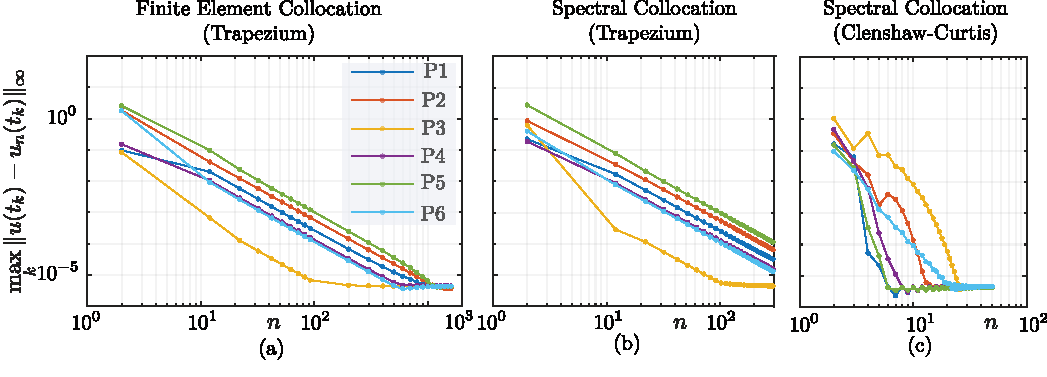
\includegraphics[width=\textwidth]{collocationConvergence}
  \caption{Convergence of (a) a Finite Element Collocation scheme with composite
    trapezium quadrature, (b) a Spectral Collocation scheme with composite trapezium
    quadrature, and (c) the same Spectral Collocation scheme with Clenshaw--Curtis
    quadrature, on test problems P1--P6.}
  \label{fig:CollTests}
\end{figure}

\begin{table}
  \caption{Parameters for test neural field problems with exact solutions.}
  \label{tab:parameters}
  \centering
  \begin{tabular}{lccccc}
    \toprule
    Problem & $D$ & $\gamma$ & $k$ & $\theta$ & $\zeta(y)$ or $\zeta_p(y)$ \\
    \otoprule
    P1      &  0.8 &  0.5 &  5     & 0.3 & $ \exp{y} \cos y  $ \\
    P2      &  -   &  -   &  -     & -   & $ y^{20} $ \\
    P3      &  -   &  -   &  -     & -   & $ (1+16y^2)^{-1}$  \\
    P4      &  -   &  -   &  -     & -   & $ \exp (-y^2) $  \\
    P5      &  -   &  -   &  -     & -   & $ \exp (-y)$  \\
    P6      &  -   &  -   &  -     & -   & $ |y|^3 $  \\
    P7p     &  -   &  -   &  -     & -   & $ \cos^2 y $  \\
    P8p     &  -   &  -   &  -     & -   & $ (1+16 \cos^2 y)^{-1}$  \\
    P9p     &  -   &  -   &  -     & -   & $ |\cos^3 y|$  \\
    P10p    &  -   &  -   &  -     & -   & $ \cos^{20} y$ \\
    \bottomrule
  \end{tabular}
 \end{table}


\appendix

% \section{Proof of \cref{lem:nemytskii}}\label{app:proof:lem:nemytskii}
\section{Proof of \texorpdfstring{\cref{lem:nemytskii}}{Lemma Nemytskii operator}}\label{app:proof:lem:nemytskii}
\begin{proof}
  Let $\XSet = C(\Omega)$. If $u \in C(\Omega)$, then by \cref{hyp:firingRate} 
  $f(u) \in C(\Omega)$ and $|f(u)| \leq \|f\|_\infty$, hence $F \colon \XSet \to
  \XSet$, $F$ is bounded, and \cref{eq:boundF} holds. To prove that $F$ is Lipschitz,
  fix $x \in \Omega$; by \cref{hyp:firingRate} and the Mean Value Theorem there exists $z(x) \in
  (u(x),v(x))$ such that 
  \begin{equation}\label{eq:interm}
    | f(u(x)) - f(v(x)) | \leq |f'(z(x))| \; | u(x) - v(x) | \leq \| f' \|_\infty |
    u(x) - v(x) |,
  \end{equation}
  thus~\cref{eq:LipF} holds with $\| \blank \| = \| \blank \|_\infty$.

  Let us now turn to the case $\XSet = L^2(\Omega)$. To prove that $F$ maps
  $L^2(\Omega)$ to itself see for instance~\cite[Lemma 3.30]{Lord:2014ir}: for any $u \in
  L^2(\Omega)$, we have
  \[
    \Vert F(u) \Vert^2_{L^2(\Omega)} = \int_\Omega |f(u(x))|^2\, dx \leq |\Omega| \;
    \Vert f \Vert^2_\infty.
  \]
  thus $F \colon L^2(\Omega) \to L^2(\Omega)$, and \cref{eq:boundF} holds. 
  % To prove the Lipschitz continuity of $F$, fix $x \in \Omega$; by
  % \cref{hyp:firingRate} and the Mean Value Theorem there exists $z(x) \in
  % (u(x),v(x))$ such that 
  % \[
  %   | f(u(x)) - f(v(x)) | \leq |f'(z(x))| \; | u(x) - v(x) | \leq \| f' \|_\infty |
  %   u(x) - v(x) |,
  % \]
  % thus $F \colon L^2(\Omega) \to L^2(\Omega)$, % and \cref{eq:boundF} holds. 
  From \cref{eq:interm} we obtain
%   \[
%     | f(u(x)) - f(v(x)) | \leq |f'(z(x))| \; | u(x) - v(x) | \leq \| f' \|_\infty |
%     u(x) - v(x) |,
%   \]
%   thus
  \[
    \begin{aligned}
      \| F(u) - F(v) \|^2_{L^2(\Omega)} & = \int_\Omega | f(u(x)) - f(v(x)) |^2 \, dx  \\
                          & \leq \| f' \|^2_\infty \int_\Omega | u(x) - v(x) |^2 \, dx \\
			  & = \| f' \|^2_\infty \| u - v \|^2_{L^2(\Omega)}
    \end{aligned}
  \]
  which gives \cref{eq:LipF}.
\end{proof}

\section{Proof of \texorpdfstring{\cref{lem:W}}{Lemma linear integral operator}}\label{app:proof:lem:W}
\begin{proof}
  The operator $W$ is clearly linear. If $\XSet = C(\Omega)$, then \Cref{hyp:domain}
  implies compactness (hence boundedness) of $W \colon C(\Omega) \to C(\Omega)$ and
  $\| W \| = \kappa_w$ (see \cite[Section 2.8.1]{atkinson2005theoretical} and
  \cite[Section 1.2]{atkinson1997}).

  We then turn to the case $\XSet = L^2(\Omega)$. By \cref{hyp:kernel} $w \in
  L^2(\Omega \times \Omega)$, hence $W$ is a Hilbert-Schmidt operator, and this
  implies the compactness of $W$ (see, for instance \cite[Section 1.2]{atkinson1997}
  or \cite[online Chapter 8]{heil2018metrics}).
  % also known (see \cite{Krasnoselskij:1963wl,Potthast:2009bd} and \cite[Lemma
  % A.2]{Faugeras:2009gn}). 
  Take $v \in L^2(\Omega)$ and set $z = Wv$. Since $w \in L^2(\Omega \times \Omega)$,
  then $w(x,\blank) \in L^2(\Omega)$ for almost all $x \in \Omega$. Thus, $w(x,\blank) v(\blank)$ is integrable
  (and $z$ well defined) for almost all $x \in \Omega$. Using
  standard definitions and the Cauchy-Schwarz inequality we have
\[
  \begin{aligned}
    \| Wu \|^2_{L^2(\Omega)} & = \int_\Omega \bigg| \int_\Omega w(x,y) u(y) \, dy \bigg|^2 \, dx  \\
	       & = \int_\Omega \langle w(x,\blank), u \rangle^2_{L^2(\Omega)} \, dx \\
	       &  \leq \int_\Omega \| w(x,\blank) \|^2_{L^2(\Omega)} \| u \|^2_{L^2(\Omega)} \, dx \\
	       & = \| u \|^2_{L^2(\Omega)} \int_\Omega \int_\Omega |w(x,y)|^2  \, dy \, dx 
	       = \| w \|^2_{L^2(\Omega \times \Omega)} \| u \|^2_{L^2(\Omega)},
  \end{aligned}
\]
which gives $\kappa_w$ when $\XSet = L^2(\Omega)$.
\end{proof}

\section{Proof of \texorpdfstring{\cref{lem:continuityN}}{Lemma Continuity of N}}\label{app:proof:lem:continuityN}
\begin{proof}
  Fix $b>0$, and consider a sequence $\{ (t_n,u_n)
  \}_{n \in \NSet} \in Q_b$ such that $(t_n,u_n) \to (t,u)$ as $n \to \infty$. We
  prove the continuity of $N$ by showing $N(t_n,u_n) \to N(t,u)$ as
  $n \to \infty$ in $\XSet$, that is, for any $\eps >0$, there exists an
  integer $m$ such that
  \[
    \| N(t_n,u_n) - N(t,u) \| \leq \eps \quad \text{for all $n \geq m$.} 
  \]
  Fix $\eps >0 $. The convergence of $(t_n,u_n)$ to $(t,u)$, the Lipschitz
  continuity (and hence continuity) of $F$ (see~\cref{lem:nemytskii}), and
  \cref{hyp:externalInput} imply the existence of
  integers $m_1$, $m_2$, $m_3$ such that
  \[
    \begin{aligned}
    & \| u_n - u \| \leq \eps / 3,%\frac{\eps}{3}  
    &&\text{for all $n \geq m_1$,}\\
    & \| F(u_n) - F(u) \| \leq \eps / (3 \kappa_w), %\frac{\eps}{3 \kappa_w} 
    &&\text{for all $n \geq m_2$,}\\
    & \| \xi(t_n) - \xi(t) \| \leq \eps / 3,%\frac{\eps}{3}, 
    &&\text{for all $n \geq m_3$,}
    \end{aligned}
  \]
  respectively, hence for all $n \geq m = \max(m_1,m_2,m_3)$.
   \[
       \| N(t_n,u_n) - N(t,u) \| \leq
     \| u_n - u \|+ \kappa_w \| F(u_n) - F(u) \|+
     \| \xi(t_n) - \xi(t) \| \leq \eps
   \]

  We now proceed to check the Lipschitz continuity of $N$. Using the Lipschitz
  continuity of $F$ (see \cref{lem:nemytskii}) we obtain
  for any $(t,u), (t,v) \in Q_b$ 
  \[
   %  \begin{aligned}
   %    \| N(t,u) - N(t,v) \| 
   %      & \leq \| u - v \| + \| W \| \| F(u) - F(v) \| \\
   %      & \leq (1 + \kappa_w \| f' \|_\infty) \| u - v \|
   %  \end{aligned}
      \| N(t,u) - N(t,v) \| 
	\leq \| u - v \| + \| W \| \| F(u) - F(v) \| 
	\leq (1 + \kappa_w \| f' \|_\infty) \| u - v \|
  \]
  therefore $N$ is Lipschitz continuous in the second
  argument, uniformly with respect to the first, because its Lipschitz constant is
  independent of $t$.
\end{proof}

\section{Proof of \texorpdfstring{\cref{thm:existenceProjCauchy}}{Existence solution Projected Cauchy}}\label{app:proof:thm:existenceProjCauchy}
\begin{proof}
  The proof follows closely the steps in \cref{lem:continuityN,thm:existence}. Let
  \[
    Q_b = 
  \{ (t,u) \in \RSet \times \XSet_n \colon |t - t_0| \leq T, \quad \| u -
    u_0 \| \leq b \}.
  \]
  The boundedness of $P_n$ implies that $P_n N \colon Q_b \to \XSet_n$ is continuous,
  and Lipschitz continuous in its second argument, uniformly with respect to the
  first. Applying Theorem 5.2.4 in \cite{atkinson2005theoretical} we obtain the
  existence and uniqueness of a solution $u_n \in C^1(J,\XSet_n)$ to
  \cref{eq:projCauchy} with initial condition $u_n(t_0) = P_n u_0 \in \XSet_n$.
\end{proof}


\bibliographystyle{siamplain}
\bibliography{test-references}
\end{document}
